% --------------------------------- Handouts ----------------------------------
% Comment out these line to generate slides
\documentclass[handout]{ctexbeamer}
\usepackage{pgfpages}
%\pgfpagesuselayout{2 on 1}[a4paper,border shrink=5mm]
\pgfpagesuselayout{4 on 1}[a4paper,border shrink=5mm,landscape]
% -----------------------------------------------------------------------------

%\documentclass[aspectratio=169]{ctexbeamer}
\usepackage{sketcher}            % tikz 绘图
\usepackage{fontset}             % 中文字体

\usetheme{AnnArbor}              % beamer 主题
\usecolortheme{beaver}           % beamer 颜色
%\usefonttheme{serif}

\bibliographystyle{plain}        % 参考文献格式

\title{勾股定理简介}
\subtitle{数学史上最重要的定理之一}
\author{佚名}
\institute{初中数学协会}
\date{\today}
\subject{勾股定理}
\keywords{勾股定理, 历史}

\begin{document}

% \begin{frame}  % 等价于 \maketitle
% \titlepage
% \end{frame}
\maketitle

\begin{frame}{目录}
\tableofcontents[pausesections]   % pausesections 逐条显示
\end{frame}

\section{勾股定理在古代}
\label{sec:ancient}

\begin{frame}{古希腊数学}

勾股定理在西方称为毕达哥拉斯定理(Pythagorean theorem 或 Pythagoras' theorem),古希腊数学家在 2000 多年前就已经发现并证明了它\cite{Kline}。\pause
\begin{itemize}
  \item<+-| alert@+>
    公元前 6 世纪,毕达哥拉斯学派发现一个法则,可以构造直角三角形的边长;
  \item<+-| alert@+>
    公元前 3 世纪,欧几里德《几何原本》使用面积法证明勾股定理。
\end{itemize}
\end{frame}

\begin{frame}{古中国数学}{定理发现}

中国在 3000 多年前就知道勾股数的概念,比古希腊更早一些。\pause

《周髀算经》的记载:\pause
\begin{itemize}[<+-| alert@+>]
  \item 公元前 11 世纪,商高答周公问:
  \begin{quote}
  勾广三,股修四,径隅五。
  \end{quote}
  \item 又载公元前 7--6 世纪陈子答荣方问,表述了勾股定理的一般形式:
  \begin{quote}
  若求邪至日者,以日下为勾,日高为股,勾股各自乘,并而开方除之,得邪至日。
  \end{quote}
\end{itemize}
\end{frame}

\begin{frame}{古中国数学}{定理证明}
有论者认为早在公元前 11 世纪商高即已证明勾股定理\cite{Qu}。完整的证明见于三国时(公元 3 世纪)赵爽对《周髀算经》的注释。
\pause
\begin{figure}
  \centering
  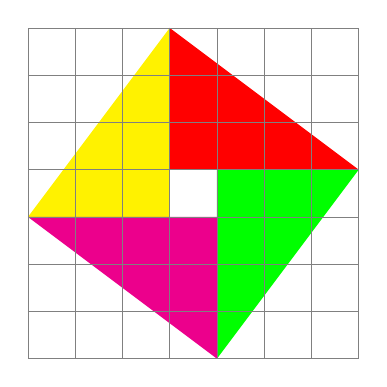
\begin{tikzpicture}[scale=0.6]
    \coordinate (A1) at (4,0);
    \coordinate (A2) at (7,4);
    \coordinate (A3) at (3,7);
    \coordinate (A4) at (0,3);
    \coordinate (B1) at (4,4);
    \coordinate (B2) at (3,4);
    \coordinate (B3) at (3,3);
    \coordinate (B4) at (4,3);
    \fill[green] (A1) -- (A2) -- (B1);
    \fill[red] (A2) -- (A3) -- (B2);
    \fill[yellow] (A3) -- (A4) -- (B3);
    \fill[magenta] (A4) -- (A1) -- (B4);
    \draw[help lines] (0,0) grid (7,7);
  \end{tikzpicture}
  \caption{弦图(赵爽《周髀算经》)}
  \end{figure}
\end{frame}

\section{勾股定理在现代}

\begin{frame}{现代叙述}
\begin{theorem}[勾股定理]
直角三角形斜边的平方等于两直角边的平方和。\pause

可以用符号语言表述为:设直角三角形 $ABC$,其中 $\angle C=90^\circ$,则有
\begin{equation}
  \label{eq:gougu}
  AB^2 = BC^2 + AC^2.
\end{equation}

\begin{center}
  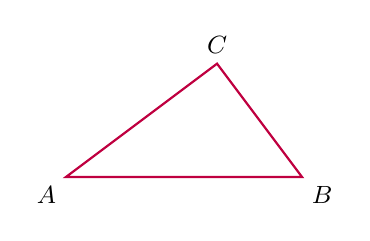
\begin{tikzpicture}[scale=0.6,font=\small]
    \coordinate (A) at (0,0);
    \coordinate (B) at (5,0);
    \coordinate (C) at (16/5,12/5);
    \draw[thick,purple] (A) -- (B) -- (C) -- cycle;
    \node[below left] at (A) {$A$}; 
    \node[below right] at (B) {$B$}; 
    \node[above] at (C) {$C$}; 
  \end{tikzpicture}
\end{center}
\end{theorem}
\end{frame}

\begin{frame}{勾股数}
满足式 \eqref{eq:gougu} 的整数称为\emph{勾股数}。第 \ref{sec:ancient} 节所说毕达哥拉斯学派得到的三元数组就是勾股数。

\begin{table}
  \centering
  \begin{tabular}{rrr}
    3 & 4 & 5 \\
    5 & 12 & 13 \\
    7 & 24 & 25 \\
    8 & 15 & 17 
  \end{tabular}
  \caption{\label{tab:triple}勾股数举例}
  \end{table}
\end{frame}

\begin{frame}{参考文献}
\nocite{Yano}
\bibliography{references}
\end{frame}

\end{document}
